\chapter{The Architecture of Dresden OCL}
\label{chapter:architecture}

\begin{flushright}
\textit{Chapter written by Claas Wilke}
\end{flushright}

This chapter introduces into the highly generic architecture of Dresden OCL.
Before the architecture is explained, some theoretical background is shortly 
presented. Further details of Dresden OCL's architecture can be found
in~\cite{braeuerEA:OCL2007} and~\cite{wilkeEA:MODELS2010}.



\section{The Generic Three Layer Metadata Architecture}
\label{architecture:genericLayers}

The \acl{OCL} is a language that is always based on another modeling language 
(usually the \acs{UML}). Without another language used for modeling, it does 
not make any sense to define constraints because \acs{OCL} is used for
constraint specification but not for modeling itself. Thus, besides \acs{OCL}, 
a modeling language is required to define a model on that \acs{OCL} constraints 
can be specified.

Each modeling language is defined in another language, its 
\keyword{Meta-Modeling Language}. For example, the \acl{UML}'s meta-model is 
defined using the \keyword{\acf{MOF}}~\cite{spec:MOF2.0}, the standardized
meta-meta model of the \acs{OMG}. The \acs{MOF} is used to describe the 
\acs{UML} meta-model that can be used to model \acs{UML} models. Generally 
spoken, each model requires a meta-model that is used to describe the model. 
The model can be instantiated by model instances (for example a \acs{UML} class 
diagram can be instantiated by a \acs{UML} object diagram). The model can be 
enriched with \acs{OCL} constraints that are defined on the model (using an 
\acs{OCL} meta-model / abstract syntax) and can then be verified for instances
of the model afterwards.

The \acs{OMG} introduced the \keyword{\acs{MOF} Four Layered Metadata
Architecture} \cite{spec:MOF2.0}\cite[p. 16ff]{spec:UML2-2Inf} that is used to 
arrange and structure the meta-model, the model, and the model's instances into 
a layered hierarchy (see Figure~\ref{pic:architecture:mofLayers}). Generally, 
four layers can be identified, the \keyword{Meta-Meta-Model Layer (M3)}, the
\keyword{Meta-Model Layer (M2)}, the \keyword{Model Layer (M1)}, and the 
\keyword{Model Instance Layer (M0)}. The latest version of \acs{MOF} allows to
define as much layers as required for a certain use
case~\cite[p.~8f]{spec:MOF2.0}. 

\begin{figure}[!t]
	\centering
	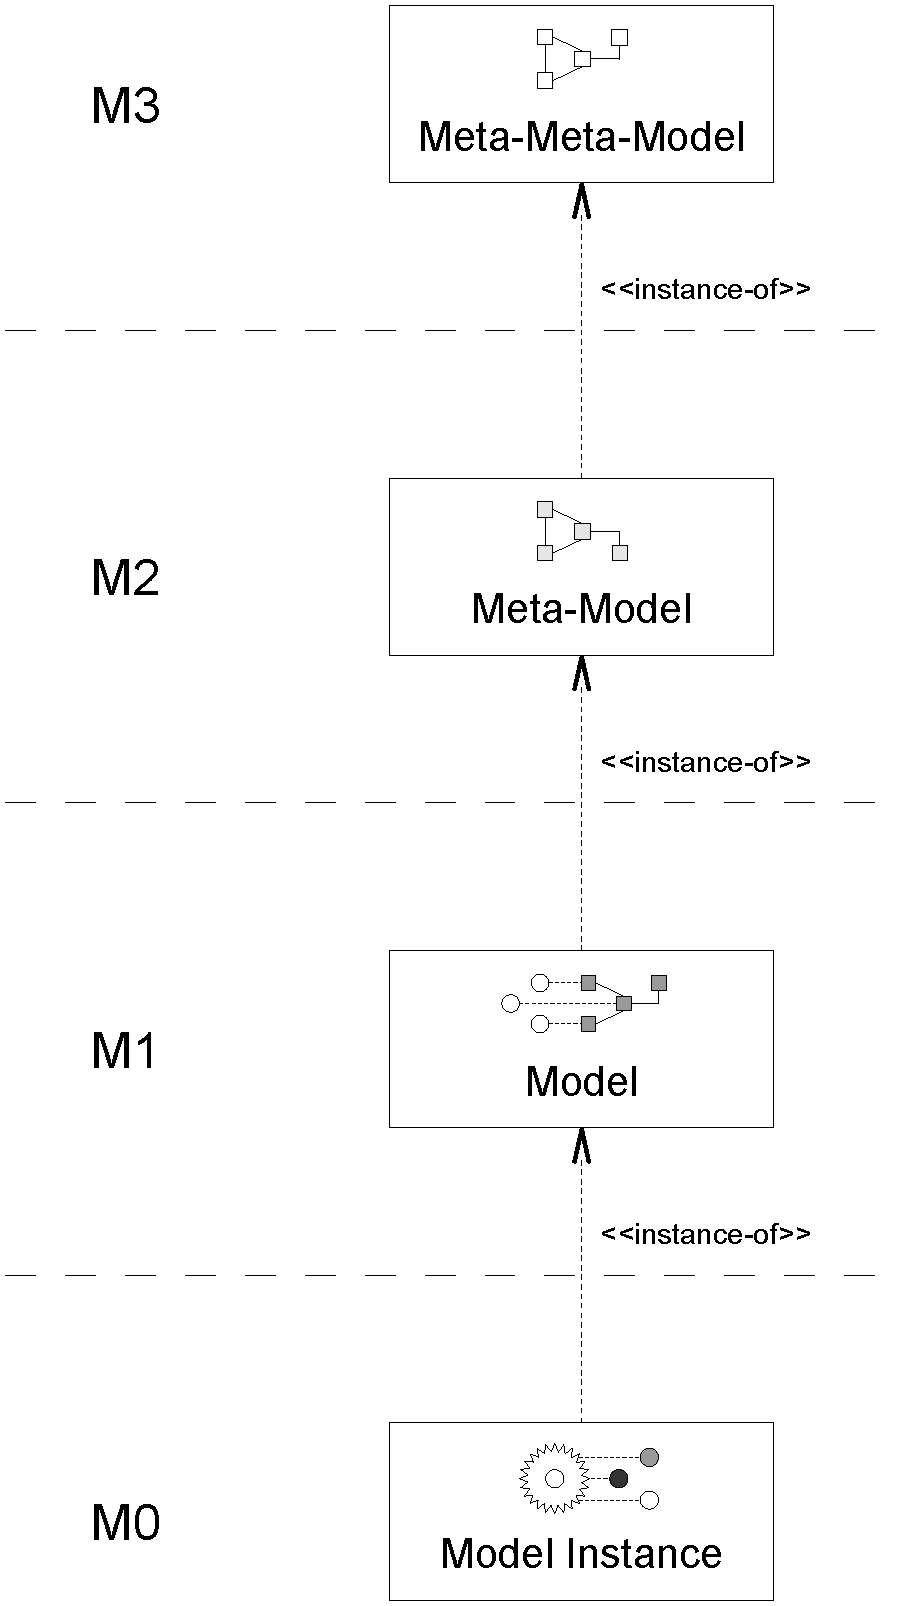
\includegraphics[width=.4\linewidth]{figures/architecture/mofLayers}
	\caption{The MOF Four Layer Metadata Architecture.}
	\label{pic:architecture:mofLayers}
\end{figure}

\begin{sidewaysfigure}[!p]
	\centering
	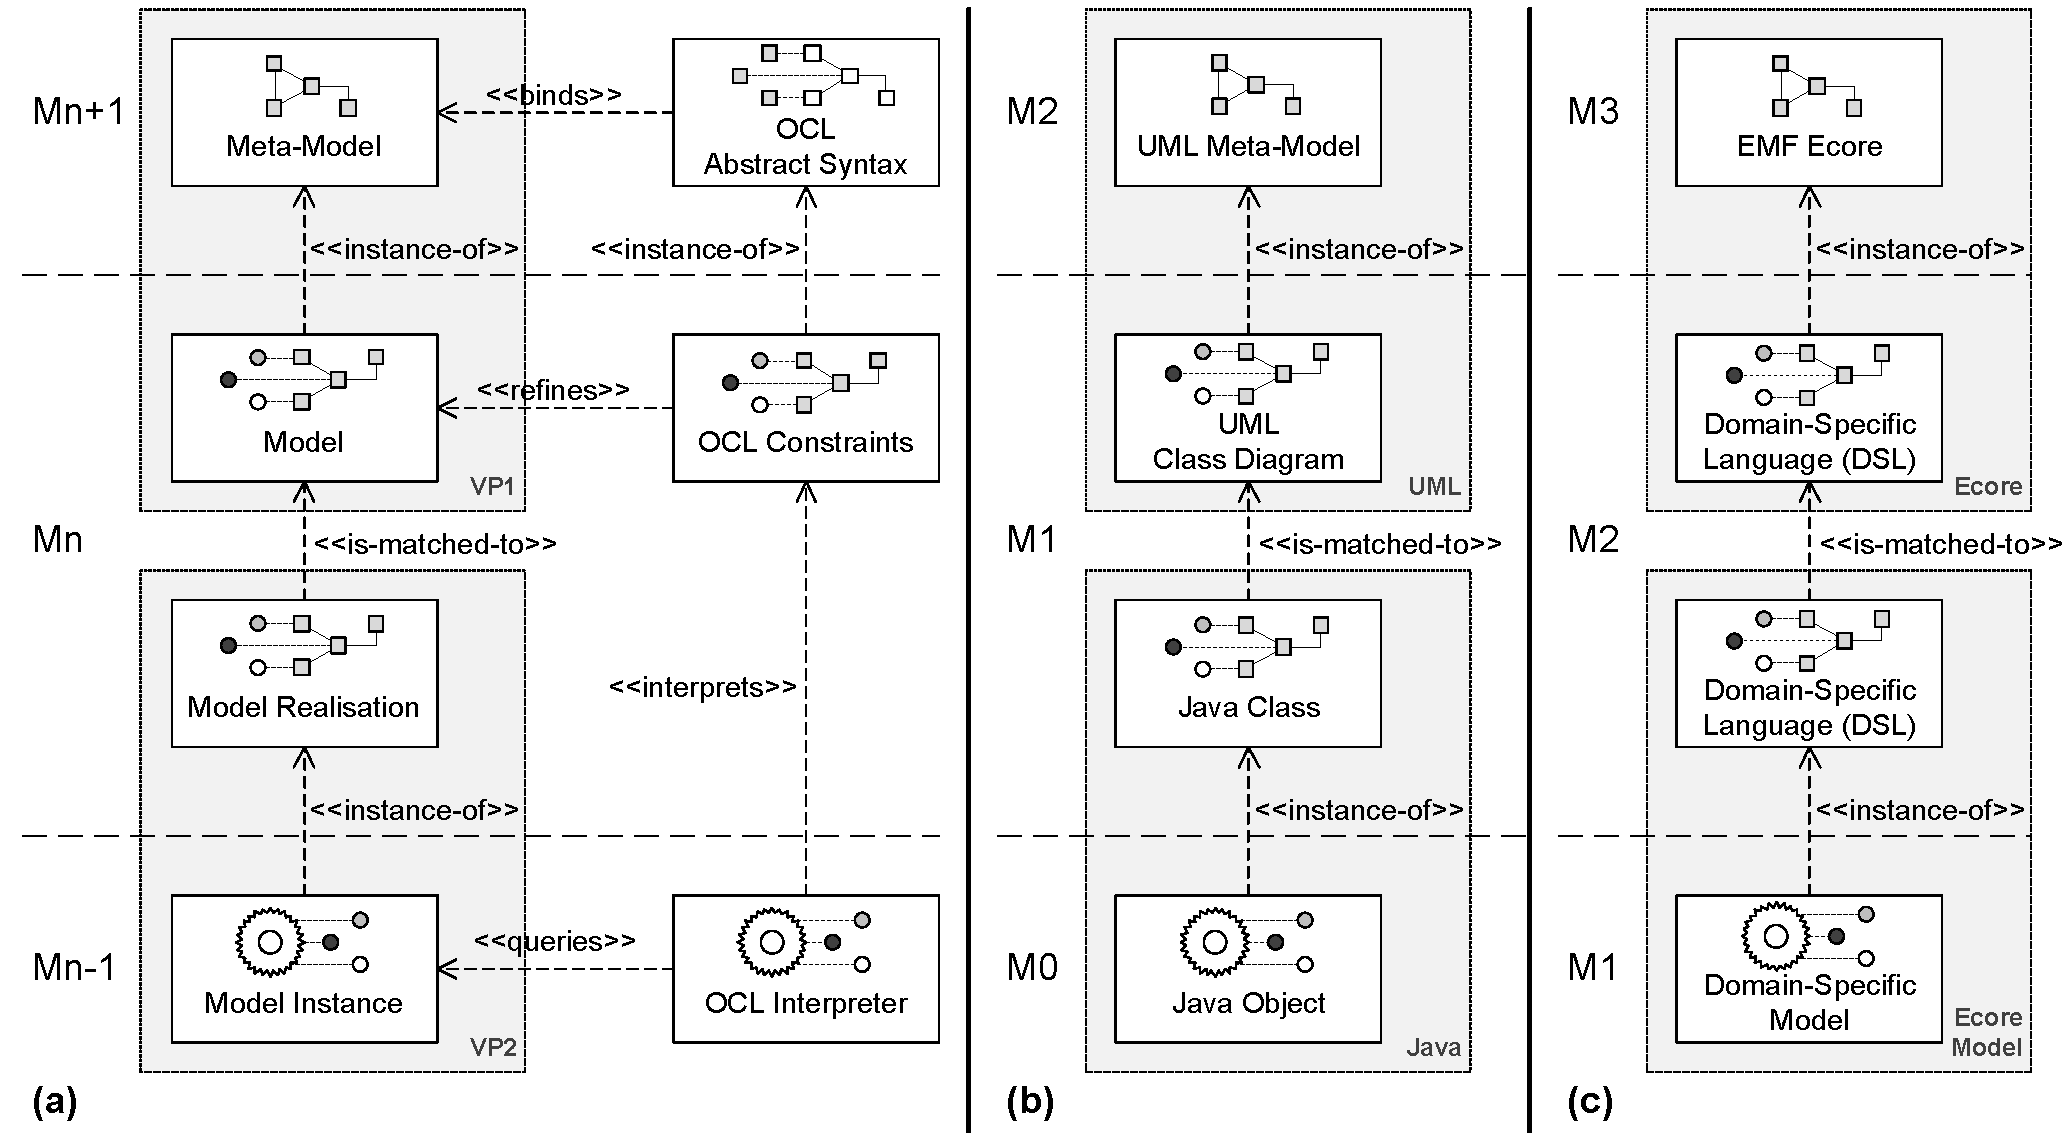
\includegraphics[width=1.0\linewidth]{figures/architecture/genericLayers}
	\caption{The Generic Three Layer Metadata Architecture.}
	\label{pic:architecture:genericLayers}
\end{sidewaysfigure}

\acs{OCL} constraints can be defined on both, meta-models and models to verify 
models or model instances, respectively. E.g., one may use \acs{OCL} to define 
rules on a meta-model that must be ensured for every model modeled with the 
meta-model. But, one may use \acs{OCL} to define rules on a model (that must be
verified for the model's instances) as well. Thus, the four layer metadata 
architecture can be generalized to a \keyword{Generic Three Layer Metadata 
Architecture}~\cite{demuth:RGWS09} in the scope of an \acs{OCL} definition (see 
Figure~\ref{pic:architecture:genericLayers}). 

On the \keyword{Mn+1 Layer} lies 
the meta-model that is used to define the model that shall be constrained. The
\acs{OCL} abstract syntax extends the meta-model to allow contexts of \acs{OCL}
constraints refering to elements of the model.

On the \keyword{Mn Layer} lies the model that is an instance of the meta-model
and can be enriched by the specification of \acs{OCL} constraints. 

Finally, on the \keyword{Mn-1 Layer} lies the model instance on that the 
\acs{OCL} constraints shall be verified. Please note that in the context of 
such a generic layer architecture, a model instance can be both a model (like a
\acs{EMF} Ecore model in Figure~\ref{pic:architecture:genericLayers}~(c))) or a
set of objects (like Java run-time objects in
Figure~\ref{pic:architecture:genericLayers}~(b)). To provide a relationship
between the model instance's elements and the model's elements a mapping is
required between both. Thus, the model instance requires a description of a
model realisation that allows to reflect on the instance's elements (e.g., for
Java run-time objects such a realisation can be considered as a set of Java
classes. Each \code{java.lang.Object} allows to reflect on its
\code{java.lang.Class}. This \code{Class} can then be mapped to the
corresponding model element in the model by comparing the \code{Class}es name
with the names of \code{Type}s existing in the model).



\section{Dresden OCL's Package Architecture}

The package architecture of Dresden OCL is shown in
Figure~\ref{pic:architecture:modules}. The architecture can be separated into
five layers: 

\begin{enumerate}
  \item The \keyword{API Layer},
  \item the \keyword{Tools Layer},
  \item the \keyword{Registry Layer},
  \item the \keyword{\acs{OCL} Layer},
  \item and the \keyword{Variability Layer}.
\end{enumerate}

\begin{figure}[!b]
	\centering
	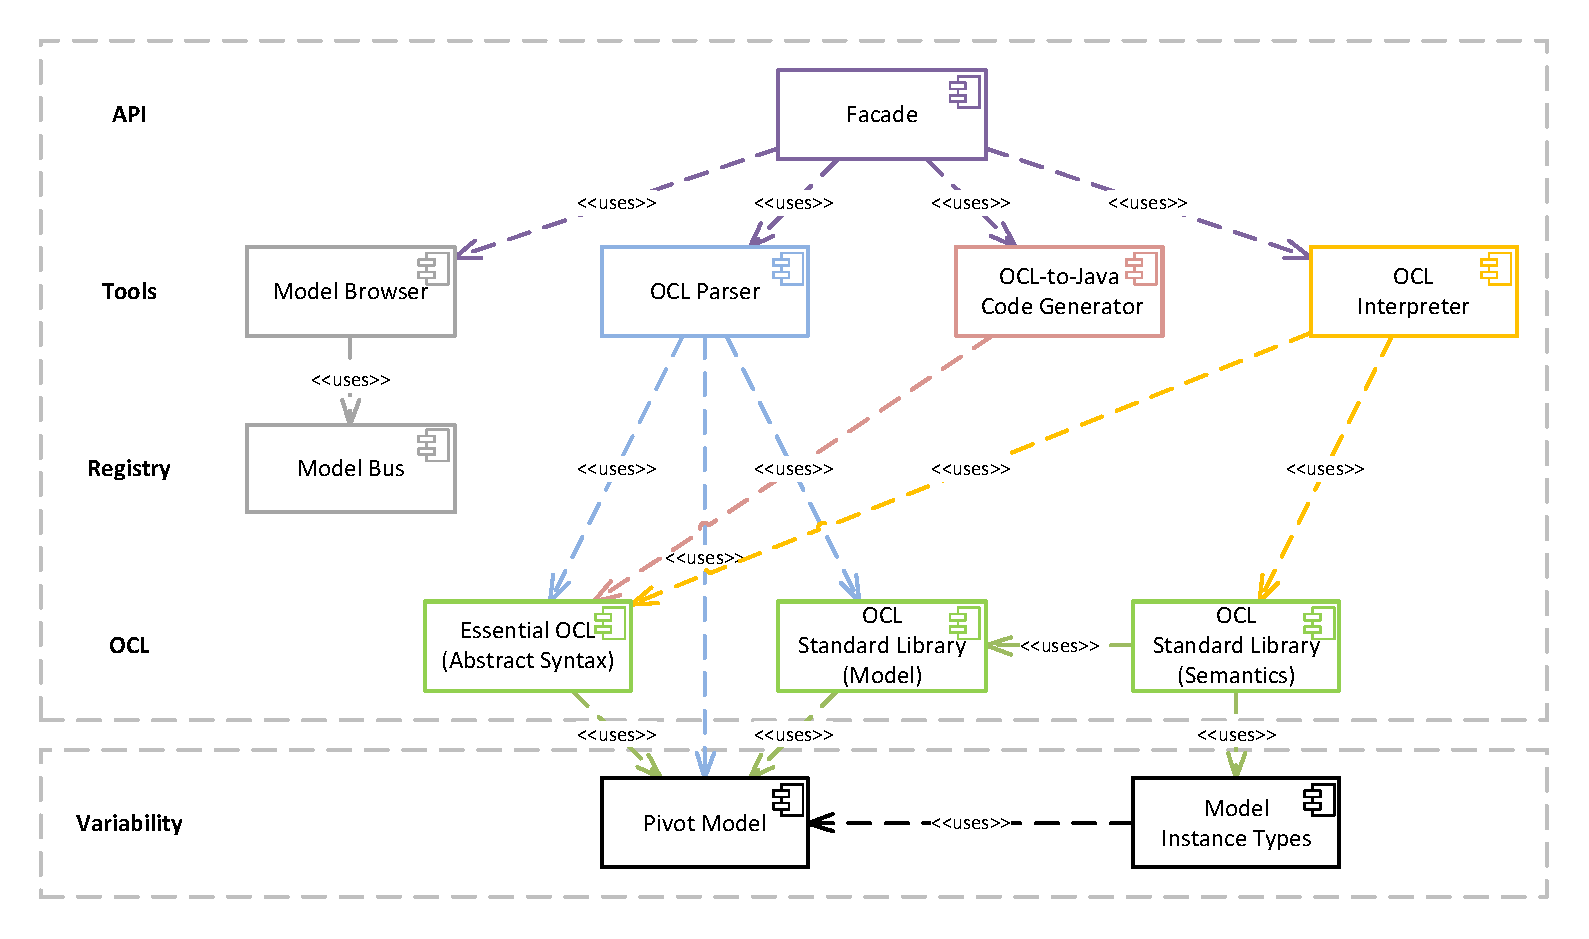
\includegraphics[width=1.0\linewidth]{figures/architecture/modules}
	\caption{The package architecture of Dresden OCL.}
	\label{pic:architecture:modules}
\end{figure}

The API layer provides the Facade of Dresden OCL that can be used by other
plug-ins to access the \acs{OCL} tools of Dresden OCL. The Facade of Dresden OCL
is introduced in Chapter~\ref{chapter:integration}.

The Tools Layer contains the Tools provided by Dresden OCL. These are: The
\acs{OCL} Parser/Editor introduced in Section~\ref{intro:oclEditor}, the
\acs{OCL} Interpreter introduced in Chapter~\ref{chapter:interpretation} and the
\acs{OCL}22Java Code Generator introduced in
Chapter~\ref{chapter:codeGeneration}. Finally, the \keyword{Model Browser} can
be used to store imported models, and model instances. The backend of the Model
Browser is the \keyword{Model Bus} that manages all meta-models and model
instance types currently provided by Dresden OCL. The model bus is located at the
Registry Layer.
%\todocw{Add OCL22SQL here when available.}

The \acs{OCL} layer contains the \acs{OCL} syntax and semantics used by the
tools of Dresden OCL. The \acs{OCL} syntax and semantics are separated into
three different packages. \keyword{Essential OCL} contains the abstract syntax
(or meta-model) of \acs{OCL} that is used by Dresden OCL and its tools. The
\keyword{OCL Standard Library Model} provides a modeled description of all
operations that are provided by the \acs{OCL} Standard Library (as defined in
\cite[Ch.~11]{spec:OCL2-2}). Finally the \keyword{OCL Standard Library
Semantics} provides an implementation of all these operations that are used by
the \acs{OCL} Interpreter of Dresden OCL for \acs{OCL} interpretation.

The last layer is the Variability Layer. The Variability layer contains the
\keyword{Pivot Model} and the \keyword{Model Instance Types} that are used to
connect Dresden OCL with various meta-models or types of model instances,
respectively. The Pivot Model is described more detailed in
Section~\ref{architecture:metaModelAdaptation}, the Model Instance Types are
explained in Section~\ref{architecture:modelInstanceAdaptation}. Further details
on both the Pivot Model and the Model Instance Types can be found 
in~\cite{braeuerEA:OCL2007} and~\cite{wilkeEA:MODELS2010}.

Dresden OCL has been developed as a set of Eclipse/\acs{OSGi} plug-ins. All
packages represent different Eclipse plug-ins. Additionally, \acl{DOT4Eclipse}
contains some plug-ins to provide \acs{GUI} elements such as wizards and 
examples to run \acl{DOT4Eclipse} with some simple models and \acs{OCL} 
expressions. An overview over all plug-ins provided with \acl{DOT4Eclipse} can
be found in Table~\ref{tab:plugins} in the appendix of this manual.



\section{Dresden OCL and the Generic Three La\-yer Me\-ta\-da\-ta Architecture}
\label{theory:DOTLayers}

\begin{sidewaysfigure}
	\centering
	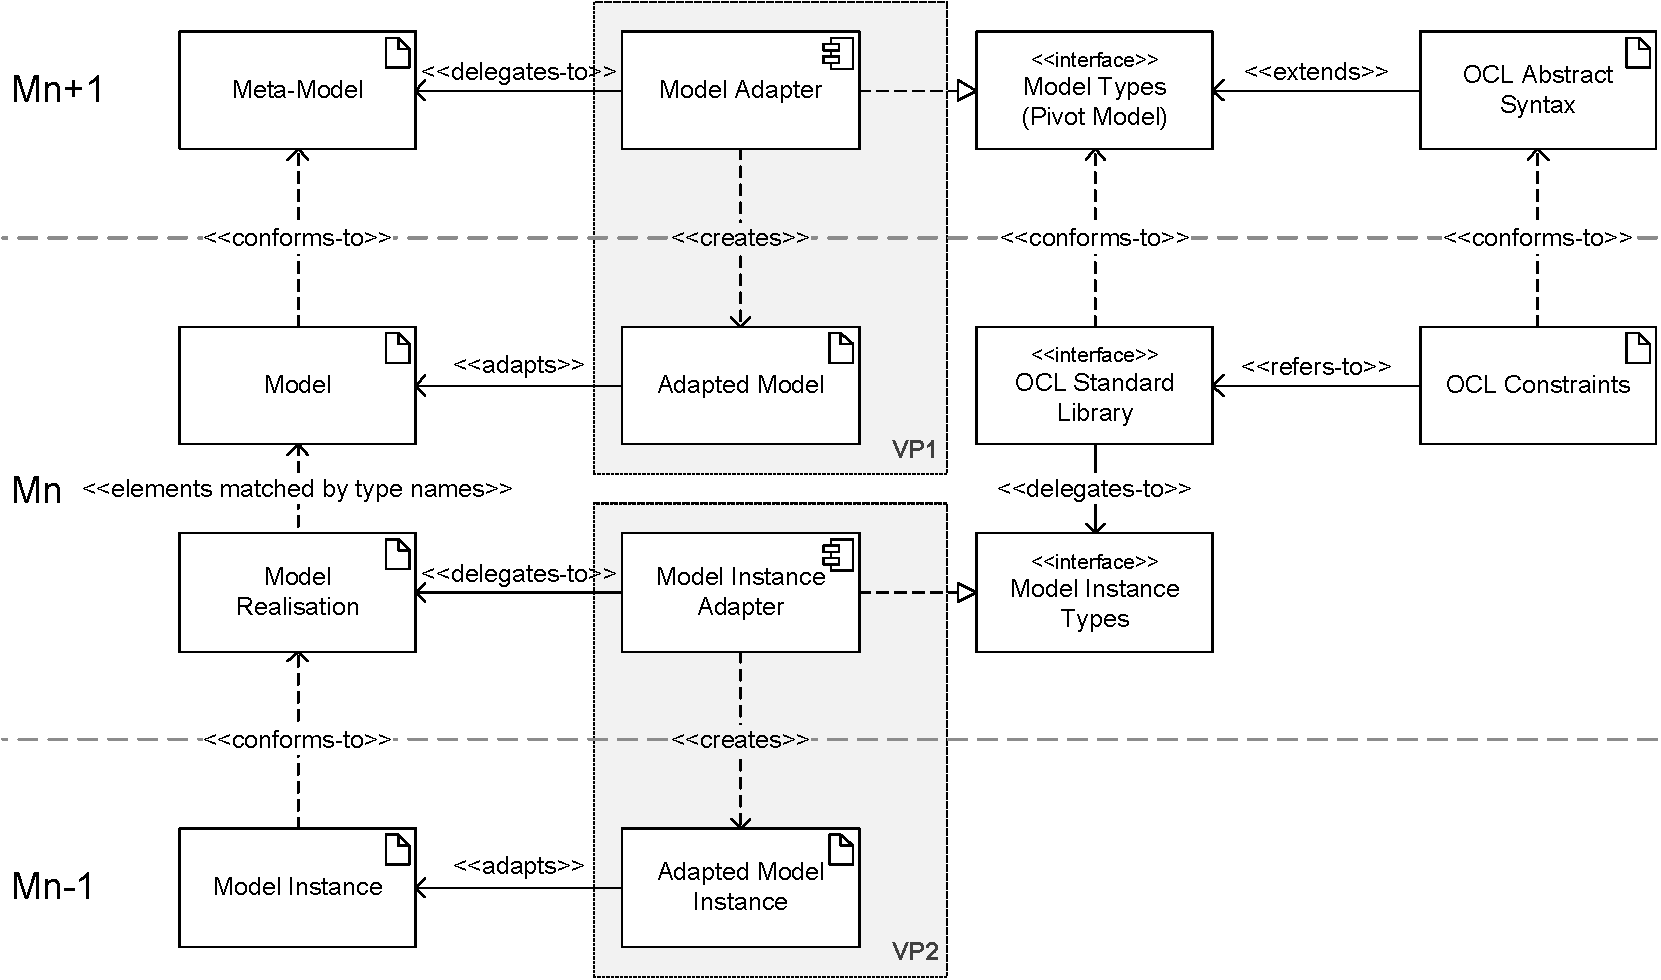
\includegraphics[width=1.0\linewidth]{figures/architecture/modeladaptation}
	\caption{The architecture of Dresden OCL with respect to the Generic Three Layer
	Metadata Architecture.}
	\label{pic:architecture:genericArchitecture}
\end{sidewaysfigure}

Figure~\ref{pic:architecture:genericArchitecture} shows the architecture of 
Dresden OCL with respect to the Generic Three Layer Metadata Architecture
(introduced in Section~\ref{architecture:genericLayers}). At the first sight, 
the architecture seems to be very complex. But do not be afraid! The 
architecture will now be explained step by step.


\subsection{The Adaptation of Meta-Models, Models and Model Instances}

As you can see, the left part of 
Figure~\ref{pic:architecture:genericArchitecture} shows the Generic Three Layer
Metadata Architecture. Meta-models, models and model instances are adapted and 
loaded into Dresden OCL. It could be argued that such an adaptation is expensive
and costly, but the opposite is the truth. The architecture of Dresden OCL allows
its users to adapt the toolkit to every meta-model and model instance type they 
want to. After the adaptation of a new meta-model or model-instance type, they
can reuse the complete set of tools provided by Dresden OCL! Thus,
to adapt the \acs{OCL} Interpreter to a new type of model instance, only one 
adaptation is required. The rest comes for free!


\subsection{How Meta-Models and Models are Adapted}
\label{architecture:metaModelAdaptation}

As already said, the core feature of Dresden OCL is the \keyword{Pivot Model}
(a.k.a. \keyword{Model Types}). The pivot model is a meta-model that abstracts
from all other meta-models. It contains interfaces to define the structural 
parts of a model such as
\code{Types}, \code{Namespaces}, \code{Operations} and \code{Properties}. 
Furthermore, these interfaces provide methods to reason on them (e.g., the 
interface \code{Namespace} provides a method \code{getNestedNamespaces()} to 
retrieve all contained \code{Namespaces}).

Every meta-model users want to work with can be adapted to the pivot model. The
\keyword{Adapted Meta-Model} must implement the interfaces of the pivot model 
and must adapt them to its meta-model elements. E.g., adapting the \acs{UML}2 
meta-model, the interface \code{Type} from the pivot model must be adapted to 
the meta-model element \code{UML2Class}. Besides the adaptation of the pivot 
model, each meta-model must provide a \code{ModelProvider} that provides 
methods to load model resources of the adapted meta-model and adapts them to 
its pivot model implementation. The result is an \keyword{Adapted Model},
Dresden OCL can work with. Further details about the adaptation of meta-models to
the pivot model can be found in Chapter~\ref{chapter:pivotModelAdaptation}.


\subsection{How Model Instances are Adapted}
\label{architecture:modelInstanceAdaptation}

If the \acs{OCL} Interpreter shall be used to interpret instances of amn opened 
model, a second adaptation is required, an adaptation to the \keyword{Model 
Instance Type Model}. The model instance type model can be considered as similar
to the pivot model, but the purpose is different. If \acs{OCL} constraints shall
be interpreted on run-time objects or values, operations and properties of these
run-time values must be accessible. E.g., if a constraint like \code{context 
Person inv: age >= 0} shall be interpreted, the property \code{age} of a
run-time object of the class \code{Person} must be accessed. The \acs{OCL} 
interpreter does not accesses this property directly, but delegates the request 
to a \keyword{Model Instance Element} adaptation to let the model instance type
become exchangeable\footnote{To be honest, the interpreter does not access the
model instance element directly but uses the \acs{OCL} standard library
semantics instead which delegate the request to the model instance element. But
this is a technical detail and not important in this context.}. Thus,
Dresden OCL contains a second model the \keyword{Model Instance Types}
that can be considered as an abstraction of all model instance types. The model 
instance types define a set of interfaces to describe the elements of a model 
instance (e.g., \code{IModelInstancePrimitiveType} and 
\code{IModelInstanceObject}). These interfaces provide operations to reflect on 
the model instance elements (e.g., the operation
\code{IModelInstanceType.invokeOperation()} or the operation 
\code{IModelInstanceElement.isTypeOf()}). The reflection mechanism can be 
considered as similar to the mechanism provided by Java in the package 
\code{java.lang.reflect}.

Each model instance type users want to work with must be adapted to the model 
instance types. Besides an adaptation of the interfaces, also a 
\code{ModelInstanceProvider} must be implemented that is responsible to adapt 
model instance objects to the implemented interfaces. Due to the fact of this 
second adaptation, Dresden OCL is able to use the same \acs{OCL} Interpreter for
different types of model instances! More details about the adaptation of model 
instances to Dresden OCL are available in 
Chapter~\ref{chapter:modelInstanceTypeAdaptation}.


\subsection{Coupling between Models and their Instances}

As mentioned above, different types of models can be connected with different 
types of instances. E.g., a \acs{UML} class diagram could be implemented by a 
set of Java Classes (and their objects) or by an \acs{XML} document. To 
maintain this loose coupling, meta-models and model implementation types do not 
know each other. If a model instance is imported into Dresden OCL, a model (and
thus also a meta-model) has to be selected, to that the instance belongs to. The
objects of the instance are matched to the types of the selected model by the 
name of their types. E.g., a Java instance's \code{Object}s are matched by
associating their \code{Class}es' names to the names of the types of the
selected model.



\section{Summary}

This Chapter introduced into the architecture and package structure of
Dresden OCL. The \keyword{Pivot Model} and the \keyword{Model Instance Types} 
have been explained shortly. Also the relationships between the pivot model, 
\keyword{Essential \acs{OCL}} and the \keyword{\acs{OCL} Standard Library} have
been presented. One may argue that the architecture seems to be complex and 
complicate. Nevertheless, it should be remembered that Dresden OCL was 
designed as generic as possible. Thus, Dresden OCL can be adapted to various
different kinds of meta-models and model instances without changing the
\acs{OCL} Parser nor the \acs{OCL} Interpreter! The currently existing
adaptations to meta-models and model instances are documented in
Section~\ref{sect:info:models} and Section~\ref{sect:info:modelinstances},
respectively.
